\documentclass{article}
\usepackage{blindtext}
\usepackage[utf8]{inputenc}
\usepackage{graphicx}
\usepackage{multicol}
\usepackage{listings}
\usepackage{url}
\author{Ruben Van Assche}
\title{Numerieke Integratie - Oefening 6}
 
\begin{document}
 \maketitle
 \begin{flushleft}
\section{Plot}
Plot de functie $f(x) = -log(1+x)*log(1-x) $ op het interval [-1,1]:
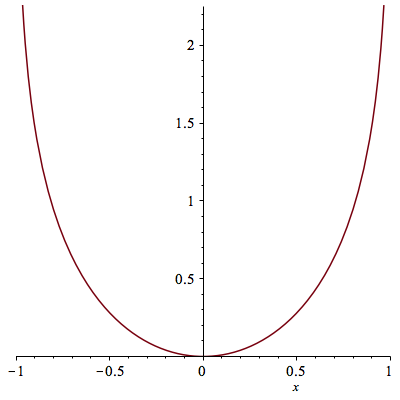
\includegraphics[scale=0.6]{Plot}

Wat meteen opvalt bij de plot van deze functie is dat de functie naar $\infty$ gaat in de punten -1 en 1.
\section{Bereken integraal met Maple}
Er wordt gevraagd de gegeven functie te integreren met Maple. Dit kan simpel via het volgende commando in Maple:
$ int(-log(1+x)*log(1-x), x = -1 .. 1) $
\newline

Dit geeft als uitkomst: $ -4+4*ln(2)-2*ln(2)^{2}+\frac{1}{3}*\pi^{2} $
\newline

Wanneer we dit numeriek uitrekenen bekomen we: 1.101550828.
\newline

Maple zal de integraal dus berekenen en een eindig getal uitkomen. Dit terwijl de grenzen van de functie waarop we integreren naar oneindig gaan en dus logischerwijs de integraal oneidig zou moeten zijn.
\section{Trapeziumregel}
We gaan nu de integraal bereken d.m.v. de trapeziumregel, we integreren over het interval [-1,1] en zullen het interval opdelen in $ 2^{k} $ subintervallen waarbij $ k = 1, 2, ...$. We noteren $T(k)$ voor de benadering.
\newline
Om de juiste k te vinden voor de juiste benadering zullen we vereisen dat de relatieve fout  $\leq 2^{-23}$.Dus:
\newline

$\frac{T(k)-T(k+1)}{T(K+1)} \leq 2^{-23}$
\newline

Via numerical recipes $\footnotetext{\url{http://e-maxx.ru/bookz/files/numerical_recipes.pdf}}$vinden we algauw een methode om d.m.v. de trapeziumregel de integraal uit te rekenen. Hierbij is a de ondergrens en b de bovengrens van de integraal.
\begin{verbatim}
Doub next() {
   	Doub x,tnm,sum,del;
   		Int it,j;
   		n++;
   		if (n == 1) {
   			   return (s=0.5*(b-a)*(func(a)+func(b)));
   		} else {
   			   for (it=1,j=1;j<n-1;j++) it <<= 1;
   			   tnm=it;
   			   del=(b-a)/tnm; 
   			   x=a+0.5*del;
   			   for (sum=0.0,j=0;j<it;j++,x+=del) sum += func(x); 
   			   s=0.5*(s+(b-a)*sum/tnm); 
   			   return s;
   		} 
}
\end{verbatim}

Deze functie heb ik herschreven zodat deze iets leesbaarder is(zie trapezium(...) in main.cpp).
\section{Probleem met grenzen}
Wanneer we nu de code uitvoeren in zijn huidige vorm, dan bekomen we een integraal die uitgerekend oneindig is. We willen natuurlijk net zoals in Maple een eindige uitkomst. Het probleem zit hem in de grenspunten -1 en 1. Namelijk:
\newline

$ -log(1+(-1))*log(1-(-1)) = \infty$
\newline
$ -log(1+1)*log(1-1) = \infty $
\newline

Vermits de trapeziumregel telkens ook rekening houdt met de grenspunten zal de uitkomst telkens oneindig zijn.
\newline

De trapeziumregel zegt:

$ \frac{b-a}{n}*(\frac{1}{2}f_{0} + f_{1} + f_{2} + ... + f_{n-1} + \frac{1}{2}f_{n}) $
\newline

Het probleem zit hem dus in $ \frac{1}{2}f_{0}$  en $ \frac{1}{2}f_{n} $. Wanneer we $ \frac{1}{2}f_{0}$  en $ \frac{1}{2}f_{n} $ aanpassen naar $ \frac{1}{2}f_{1}$  en $ \frac{1}{2}f_{n-1} $ zullen we wel een resultaat krijgen dat eindig is. Deze punten liggen zeer dicht tegen de originele grenspunten en zullen steeds dichter gaan liggen tegen de originele grenspunten naarmate het aantal deelintervallen groeit.
\newline

Grafisch:
\newline
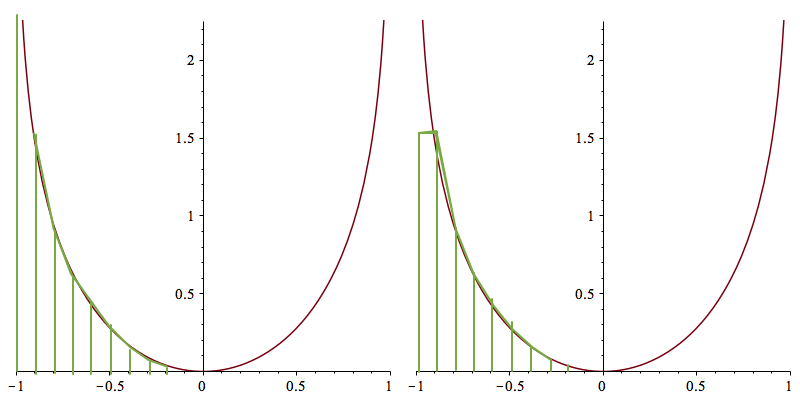
\includegraphics[scale=1.5]{Plot2}
\newline

We zullen dus nu geen trapezia meer gebruiken op de grenzen van het interval maar rechthoeken.

\section{Efficiëntie}
Wanneer we nu de integraal berekenen, dan krijgen we een eindig getal. Maar vermits onze deelintervallen telkens verdubbelen wordt het aantal keer dat we f(x) berekenen drastisch groter. Het probleem met de huidige vorm van de trapeziumregel is dat bij elke vergroting van k we een hoop punten opnieuw moeten berekenen. We roepen dus meerdere malen f(x) op met dezelfde x-coordinaat.
\newline

Wanneer we de trapeziumregel uitschrijven voor a = -1 en b = 1 en h = $\frac{a-b}{2}$(normaal gedeeld door n maar voor dit voorbeeld houden we hier de n constant op 2) met:
\newline
\textbf{n=2} 
\newline
$h(\frac{1}{2}f(-1)+\frac{1}{2}f(1)) + h(f(0))$
\newline
\textbf{n=4} 
\newline
$\frac{h}{2}(\frac{1}{2}f(-1)+\frac{1}{2}f(1)) + \frac{h}{2}(f(0)) + \frac{h}{2}(f(-0.5) + f(0.5))$
\newline
\textbf{n=8} 
\newline
$\frac{h}{4}(\frac{1}{2}f(-1)+\frac{1}{2}f(1)) + \frac{h}{4}(f(0)) + \frac{h}{4}(f(-0.5) + f(0.5)) + \frac{h}{4}(f(-0.75) + f(-0.25)+f(0.25) + f(0.75))$
\newline

Wat opvalt is dat bij elke vergroting van n de volledige uitdrukking van de vorige n opnieuw voorkomt maar dan gedeeld door 2. Vervolgens worden er nog enkele termen f(x) bijgeteld. Dit vanaf n = 4.
\newline

Het aantal termen dat extra berekend worden hangt af van n. Voor n zijn er namelijk $ 2^{log_{2}(n)-1}$. De eerste 2 termen zullen altijd f(a+h) en f(b-h). De termen daarop zullen altijd in koppel de regel volgen namelijk f(a+h+2*ih) en f(b-h-2ih) voor i = 1 ... $  \frac{2^{log_{2}(n)-1}-2}{2}$.
\newline

Voor n = 8 bekomen we dan f(-0.75), f(-0.25), f(0.25), f(0.75).
\newline

Voor elk niveau n tellen we deze termen op en vermenigvuldigen we ze met $\frac{b-a}{n}$. Wanneer we dan (zoals eerder aangehaald) de uitdrukking van het niveau n/2 erbij optellen en delen door 2, bekomen we de trapeziumregel voor niveau n.
\newline

Vermits we bij deze opgave telkens de n verhogen(en dus telkens al het vooraande niveau van de trapeziumregel hebben berekend) zorgt deze techniek ervoor dat het algoritme een stuk sneller zal werken.
\section{Uitkomsten}

\begin{tabular}{l l c r }
  k & n & uitkomst & fout \\
  2 & 2 & 0.281046996500607548785666267577  &  0.498593093473180648533826797575\\
  3 & 4 & 0.560516803502735250219757290324  & 0.269635219274728110683270188019  \\
  4 & 8 & 0.76744774432596130075978635432  & 0.150459596214987223472547839265 \\
  5 & 16 & 0.903368151657886198080404938082 &0.0848389756740937223122855925794  \\
  6 & 32 & 0.987113882306442702585513870872  &  0.047856810225218586463125092223\\
  7 & 64 &  1.03672839642946268412515564705 & 0.026873532299304198067702031949 \\
  8 & 256 &  1.06535833813979552431305819482 & 0.0149890082226010294685902834999 \\
  9 & 512 & 1.08156999975950940395819088735  & 0.00829790115354625198995641710553 \\
  10 & 1024 & 1.0906198555166817243389232317  & 0.00455971569647120166662856988182 \\
  11& 2048 & 1.09561555094160811840708902309 & 0.00248817125778888091278129301998  \\  
  12 & 4096   & 1.09834842993601244920398585236  &0.00134916633349519755370737872369  \\ 
   13 & 8192  &  1.09983228662962417843118601013 & 0.000727408525770914678697243171968 \\ 
  14 & 16384   & 1.10063289638219652388784197683  &0.000390203210223912053816741618562  \\ 
  15 & 32768   &  1.10106253451782265528891002759 &0.000208376771486195184720016659874  \\ 
  16 & 65536   & 1.10129201819303723652865301119  & 0.000110833515117285673649491495318 \\ 
   17 & 131072  & 1.10141409178842986094082334603  &5.87415121914734098939464557176e-05  \\ 
  18 &  262144  &  1.10147879431845496789321714459 & 3.10337624305036046627043200274e-05 \\ 
   19 &  524288 & 1.10151297841054107706781906018  &1.63485632969174115398588997827e-05  \\ 
  20 &  1048576  &  1.10153098685960326719168733689 &8.59017323862922101737182173364e-06  \\ 
   21 & 2097152  & 1.10154044928289196469961552793 & 4.50304665036797858448328751857e-06 \\ 
   22 &  4194304 &1.10154540959325886184672071977  & 2.35550720157963513944824988922e-06 \\ 
   23 & 8388608  & 1.10154800429751587032001225452 &1.22974669900919639577185123874e-06  \\ 
   24 & 16777216  & 1.10154935892420380305622984451 &6.40870198210446683313105519647e-07  \\ 
   25 & 33554432  & 1.10155006487481221810753595491 & 3.33433604822107665357821875904e-07 \\ 
   26 & 67108864  & 1.10155043216874370948232808587 &1.73215997301873115617892612966e-07  \\                                                                                           
   27 & 134217728  & 1.10155072195731307260757603217 & 8.98573053904804712807016060447e-08 \\                                                                                           
\end{tabular}
\newline

Wanneer we dus k = 27 en dus n = 134217728 hebben we een fout 8.98573053904804712807016060447e-08 $\leq 2^{-23}$
\section{Code}
\lstinputlisting{main.cpp}


\end{flushleft}
\end{document}